\section{Diagrama de Objetivos (1.3)}

\subsection{Descripci\'on: Conteo}


El presidente de mesa abre la urna y pone a la máquina impresora de voto en “Modo de conteo”, dando así comienzo al conteo de cada voto. En caso de que no haya nada impreso, o haya algo escrito a mano, se impugna el voto.

Cuando la máquina lee el chip, lleva la cuenta de los votos procesados. Al pasar la boleta por la máquina, figura en la pantalla el voto grabado. Se verifica que lo leído por el lector del chip, coincida con lo impreso en el papel. Los fiscales observan con detenimiento.\\

En caso de que ocurra alguna irregularidad, el presidente de mesa y/o fiscales lo comunicarán al fiscal general de la escuela. Frente a esta irregularidad, el fiscal general podrá anular la mesa (si lo considera necesario), por lo que no se enviaría el resultado al centro de Cómputos.\\

Al finalizar el conteo, el presidente de mesa insertará una boleta vacía en la máquina impresora de voto, la cual grabará en el chip los resultados contabilizados de la mesa. Además imprimirá con tinta en la boleta los ganadores de cada categoría para así obtener una manera de contrastar lo grabado con lo contabilizado.
Luego, el presidente de mesa llevará la boleta con el conteo al Fiscal general, quien será el encargado de cargarla en la máquina de impresión de votos con conexión telefónica destinada al envío de resultados. El mismo posee dos contraseñas; al ingresar la primera, la máquina impresora de votos le permitirá ingresar al “Modo envío”. Una vez cargadas todas las boletas, las envía por el enlace telefónico al centro de cómputos nacional, enviándole también su contraseña única de Fiscal General. El presidente de mesa podrá acompañarlo en todo momento para ver que se contabilice lo correcto.\\
\textcolor{red}{El fiscal general puede, en todo momento, utilizar el pendrive suministrado por el Ministerio, para chequear que el código que se ejecuta en cada máquina, es el correcto.}\\
Posteriormente, el presidente de mesa inserta la boleta con el conteo impreso en la urna junto a todas las boletas contabilizadas de la mesa. El presidente sella la urna, el fiscal general la agrupa con las otras que hay en escuela, y brinda al correo todas las urnas de su escuela e identifica a las urnas que hayan sido impugnadas. Además, envía el padrón para poder identificar a quienes votaron. El correo se encarga de enviarlas al centro de cómputos nacional.\\

El Sistema del Centro de Cómputos sólo contabilizará resultados de mesas que hayan sido cargados con contraseñas de Fiscal General válidas y correspondientes a las mesas de las urnas recibidas.
El Centro de Cómputos nacional calcula los resultados provisorios de las elecciones (como si hay ballotage, o la cantidad de diputados mediante el método D’Hont) con la información recibida por el enlace telefónico.

A las 20hs el Centro de Cómputos nacional publica los resultados del conteo provisorio en su página web.\\

Finalmente, el correo llevará todas las urnas al centro de cómputos nacional donde se realizará el conteo definitivo (No es posible saber a priori cuándo ocurrirá esto).

\newpage
\subsection{Diagrama}

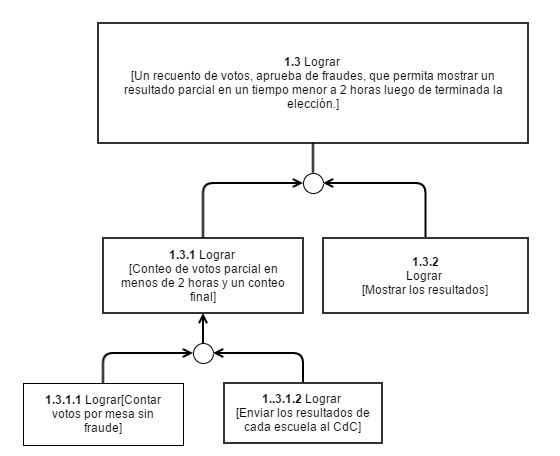
\includegraphics[scale=0.55]{imagenes/Diagramas/13/13.png}
\\
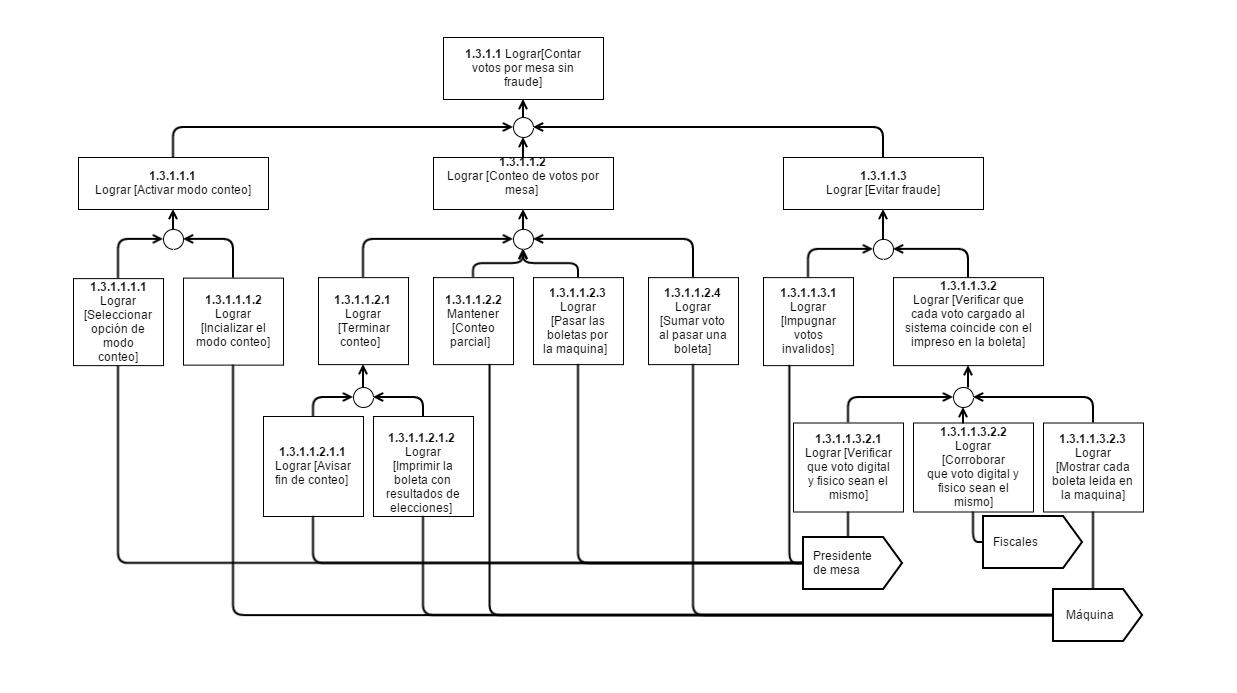
\includegraphics[scale=0.55]{imagenes/Diagramas/13/1311.png}
\\
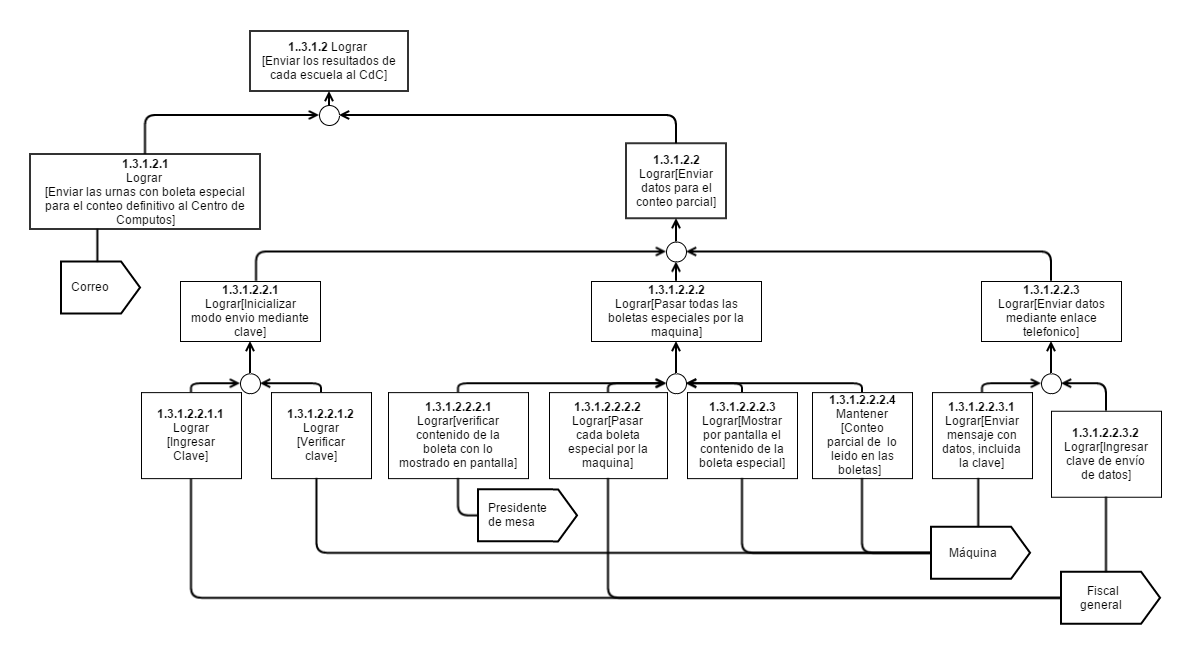
\includegraphics[scale=0.55]{imagenes/Diagramas/13/1312.png}
\\
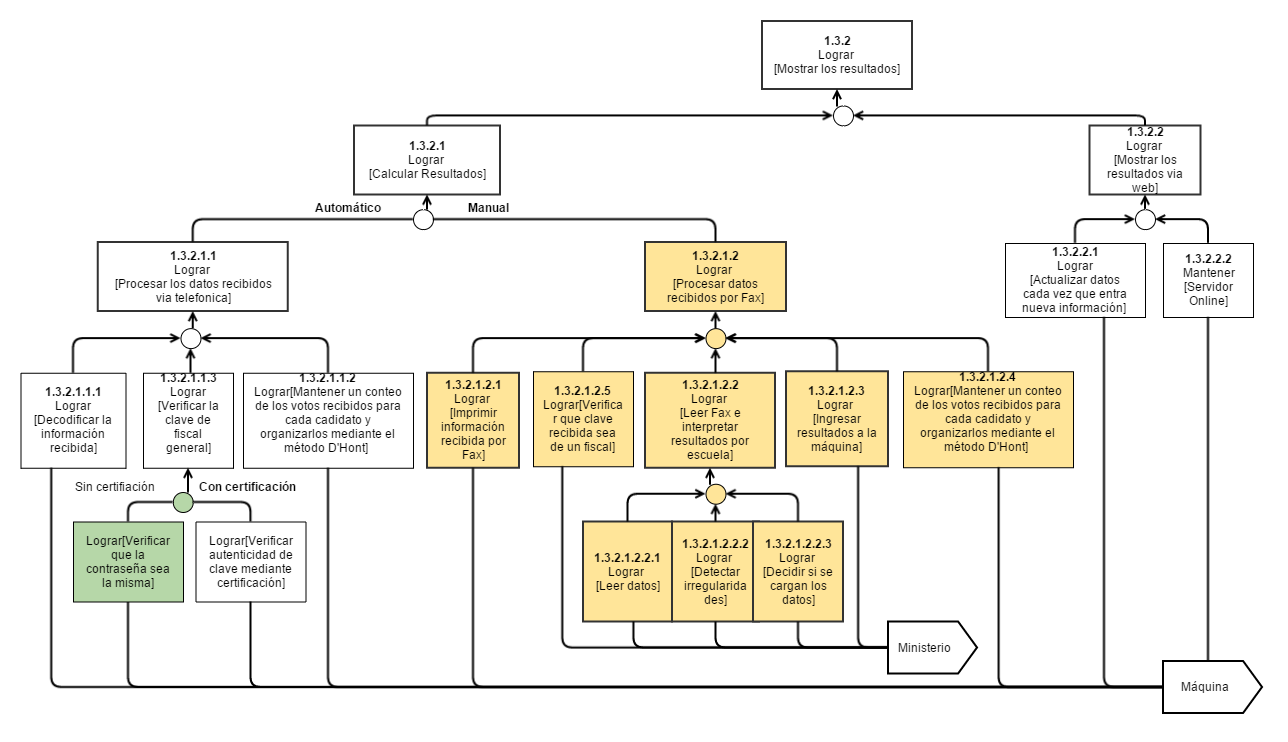
\includegraphics[scale=0.53]{imagenes/Diagramas/13/132.png}

\newpage
\subsection{Requerimientos de la m\'aquina}

Dada esta sección podemos obtener los siguientes requerimientos para nuestra maquina:
\begin{itemize}
\item Incializar Modo conteo
\item Sumar votos al pasar una boleta en modo conteo
\item Mantener un conteo parcial en modo conteo
\item Mostrar cada boleta leida en pantalla
\item Imprimir boleta especial para envio
\item Verificar clave para entrar en modo envio
\item Mantener un conteo parcial en el modo envio
\item Mostrar el contenido de la boleta especial
\item Enviar mensaje con los datos para el conteo parcial con la clave del fiscal general encriptada
\item Decodificar la información del mensaje
\item Mantener un conteo parcial de los datos recibidos para cada candidato y organizarlo según el método d'Hont
\item Verificar la clave del fiscal
\item Actualizar los resultados cuando entran datos
\item Mantenerse online
\end{itemize}